\chapter{Introducción}
\label{cap:introduccion}

\section{Descripción general y contexto}
\label{sec:intro_contexto}

Hoy en día, gran parte de la actividad de una organización pasa por la red. Esto hace que el tráfico sea cada vez más grande y más difícil de revisar, pero también que los ataques tengan más superficie sobre la que actuar. En una misma red pueden convivir tráfico de red normal con escaneos, intentos de acceso, equipos comprometidos o campañas automatizadas. Revisar todo ese tráfico mirando el contenido de cada comunicación no es realista a gran escala, tanto por volumen como por privacidad. Por eso es habitual trabajar con metadatos de flujo: en lugar de analizar directamente lo que se envía, se resume cada comunicación indicando quién habla con quién, por qué puerto, durante cuánto tiempo y cuántos paquetes y bytes se intercambian. Este tipo de información es la que se recoge habitualmente mediante tecnologías de flujo como NetFlow \cite{rfc3954}, y es la base sobre la que se desarrolla este trabajo.

El problema es que un ataque suele representar una parte muy pequeña dentro de una cantidad enorme de tráfico normal. La detección de anomalías parte precisamente de esa idea: en vez de buscar únicamente firmas concretas de ataques ya conocidos, intenta reconocer comportamientos que se salen de lo esperado \cite{garciateodoro2009anomaly}. Este enfoque es interesante porque una red real no siempre se enfrenta a amenazas idénticas a las que ya se han visto antes. Sin embargo, detectar una anomalía no es suficiente por sí solo. Si un sistema marca una traza como sospechosa, pero no explica qué ha visto para tomar esa decisión, la alerta pierde parte de su utilidad. En la práctica, el analista necesita saber si la alerta tiene sentido, qué patrón la ha provocado y si puede tratarse de un falso positivo. Por eso, en este TFG no se busca solo clasificar tráfico, sino avanzar hacia una detección explicativa.

Este Trabajo de Fin de Grado aborda la detección explicativa de anomalías en tráfico NetFlow utilizando el dataset UGR'16 \cite{ugr16}. Este conjunto de datos permite estudiar tráfico real etiquetado con distintas familias de ataque y analizar cómo se comporta cada una de ellas. A partir de este dataset, el trabajo se apoya en modelos de lenguaje, especialmente NotebookLM, para estudiar el tráfico, interpretar patrones y formular hipótesis sobre las señales que caracterizan a cada ataque. Su papel es ayudar en el análisis, la interpretación y la documentación del comportamiento observado. La detección final la realiza un clasificador contextual basado en reglas conductuales, cuya versión final hemos denominado v5.

El clasificador desarrollado no utiliza aprendizaje automático supervisado para tomar sus decisiones, ni se apoya en direcciones IP concretas. La idea es detectar patrones de comportamiento: muchos destinos contactados por un mismo origen, concentración de tráfico hacia un servicio, actividad distribuida entre varios orígenes o flujos muy ligeros repetidos en poco tiempo, entre otros casos. De esta forma, cada decisión puede acompañarse de una explicación basada en las señales que se han activado. Además, el proyecto incluye una aplicación web interactiva que permite explorar las familias de ataque, generar ventanas sintéticas de ejemplo, consultar información asociada a cada ataque y ejecutar el clasificador sobre ficheros pequeños. La web no sustituye a la evaluación experimental, pero ayuda a entender y probar el funcionamiento del sistema de una forma más visual.

Este planteamiento no significa que todos los ataques se resuelvan con la misma facilidad. Algunas familias presentan patrones claros en los metadatos NetFlow, mientras que otras son más difíciles de separar del tráfico normal porque la información disponible es limitada. Esta diferencia es importante y se tendrá en cuenta durante toda la memoria. El objetivo no es presentar el sistema como una solución perfecta, sino estudiar hasta dónde puede llegar un enfoque explicativo basado en reglas conductuales, apoyado por LLMs durante el análisis y validado sobre datos reales.

\begin{figure}[ht]
\centering
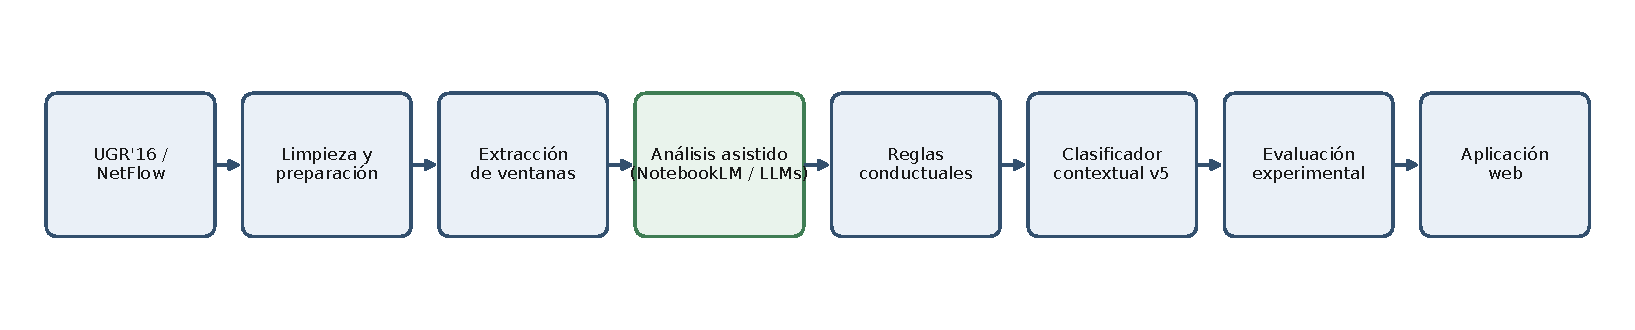
\includegraphics[width=\textwidth]{imagenes/fig_pipeline_general.pdf}
\caption{Visión general del flujo de trabajo del proyecto, desde las trazas NetFlow de UGR'16 hasta el clasificador contextual y la aplicación web.}
\label{fig:pipeline_general}
\end{figure}

\section{Motivación}
\label{sec:intro_motivacion}

La motivación principal de este TFG nace de un problema bastante claro: en una red real hay muchísima actividad y no toda tiene la misma importancia. La mayor parte del tráfico suele ser normal, pero dentro de ese volumen pueden aparecer comportamientos anómalos que interesa detectar cuanto antes. El problema es que esos comportamientos no siempre aparecen de forma evidente. Un ataque puede estar formado por muchas trazas pequeñas, por conexiones repartidas en el tiempo o por patrones que solo tienen sentido cuando se miran en conjunto. Por eso, detectar anomalías en tráfico de red no consiste simplemente en buscar una fila rara dentro de una tabla, sino en entender qué comportamiento está apareciendo dentro de una ventana de tráfico.

Además, en ciberseguridad no basta con que un sistema diga que algo es sospechoso. Si una herramienta genera una alerta pero no explica por qué, el resultado puede ser difícil de aprovechar. El analista necesita saber qué ha visto el sistema: si se trata de muchos destinos contactados por un mismo origen, de demasiadas conexiones hacia un servicio concreto, de tráfico muy repetitivo o de cualquier otra señal relevante. Una alerta sin explicación obliga a revisar manualmente el caso y puede terminar generando desconfianza, sobre todo si hay falsos positivos. Por eso, uno de los puntos que más motiva este trabajo es la explicabilidad: no solo asignar una etiqueta, sino poder justificar la decisión de una forma entendible \cite{rudin2019stop}.

Muchos enfoques de detección se basan en modelos de aprendizaje automático \cite{buczak2016survey}. Estos métodos pueden ser muy útiles y, de hecho, en este TFG se utilizan como comparación experimental. Sin embargo, no siempre es sencillo entender por qué un modelo ha tomado una decisión concreta, especialmente cuando se trabaja con modelos más complejos. En este trabajo se ha buscado una línea distinta: construir un clasificador basado en reglas conductuales, donde cada regla represente una señal del comportamiento del tráfico. La idea no es competir únicamente por obtener una métrica alta, sino conseguir que el resultado sea interpretable. Si el sistema marca una traza como ataque, debe poder explicar qué señales han llevado a esa decisión.

El uso de NetFlow también forma parte de la motivación. Trabajar con flujos permite analizar comunicaciones de red sin acceder al contenido real que se transmite, lo que resulta útil tanto por volumen como por privacidad \cite{rfc3954}. Aun así, esta forma de trabajar tiene limitaciones. NetFlow no permite ver el contenido de un correo, el payload de una conexión o la intención exacta de un usuario. Solo ofrece metadatos. Esto hace que algunas familias de ataque sean más fáciles de caracterizar que otras. Precisamente por eso resulta interesante estudiar hasta dónde se puede llegar usando solo este tipo de información, y en qué casos el enfoque se queda corto.

En este contexto, los modelos de lenguaje y NotebookLM se utilizan como apoyo durante el análisis. Su papel no es sustituir al clasificador ni decidir qué es ataque y qué no lo es. La motivación de usarlos está en que ayudan a revisar documentación, resumir patrones, comparar ventanas de tráfico y formular hipótesis que después se transforman en reglas comprobables. Es decir, los LLMs sirven como una herramienta de apoyo al razonamiento, pero la detección final sigue estando controlada por un algoritmo explícito. Esta separación es importante porque permite aprovechar la capacidad explicativa de los modelos de lenguaje sin dejar que el sistema dependa de una respuesta generada sin control.

Por último, la aplicación web surge como una forma de hacer que el trabajo no se quede solo en scripts, ficheros CSV y tablas de resultados. La web permite explorar cada ataque, ver qué señales utiliza el detector, generar ventanas sintéticas de ejemplo y ejecutar el clasificador sobre ficheros pequeños. Esto ayuda a entender el sistema desde fuera, no solo a evaluarlo numéricamente. En un trabajo de este tipo, donde la explicación es una parte central, poder visualizar y probar el funcionamiento del detector es casi tan importante como tener los resultados en tablas. Aun así, la motivación no es presentar una herramienta cerrada y perfecta, sino construir una base sólida que permita analizar qué familias de ataque se pueden detectar bien con NetFlow, cuáles siguen siendo difíciles y qué líneas de mejora quedan abiertas.

\section{Objetivos}
\label{sec:intro_objetivos}

\subsection{Objetivo general}
\label{sec:intro_obj_general}

El objetivo general de este Trabajo de Fin de Grado es diseñar, implementar y evaluar un sistema de detección explicativa de anomalías en tráfico NetFlow sobre el dataset UGR'16. El sistema se apoya en modelos de lenguaje y en NotebookLM durante la fase de análisis, pero la detección final no la realizan estos modelos, sino un clasificador contextual basado en reglas conductuales interpretables. La meta no es alcanzar una detección perfecta ni una generalización universal, sino estudiar hasta dónde puede llegar este enfoque sobre datos reales, dejando claro qué decisiones toma el sistema y por qué.

\subsection{Objetivos específicos}
\label{sec:intro_obj_especificos}

Para alcanzar el objetivo general se plantean los siguientes objetivos específicos:

\begin{enumerate}
  \item Estudiar el dataset UGR'16, comprendiendo su origen, su estructura y la forma en que están etiquetadas las distintas familias de ataque.
  \item Preparar y limpiar los datos NetFlow, dejándolos en un formato adecuado para el análisis posterior.
  \item Analizar el comportamiento de las distintas familias de ataque presentes en el dataset, identificando qué las distingue del tráfico normal.
  \item Extraer ventanas temporales de tráfico que contengan cada ataque junto con su contexto, de modo que el comportamiento pueda estudiarse en conjunto y no traza a traza de forma aislada.
  \item Emplear NotebookLM y modelos de lenguaje como apoyo al análisis, para interpretar patrones y formular hipótesis sobre las señales de cada ataque, sin que estos modelos tomen la decisión de detección.
  \item Diseñar reglas conductuales explicables a partir de esas hipótesis, de manera que cada regla represente una señal medible del comportamiento del tráfico.
  \item Implementar el clasificador contextual final, que integra esas reglas y añade un análisis global por origen para detectar comportamientos repartidos en el tiempo, como el escaneo horizontal por SSH.
  \item Evaluar los resultados del clasificador mediante métricas adecuadas (precisión, recall y F1, entre otras), familia por familia.
  \item Comparar el enfoque con modelos de Machine Learning clásico, utilizados como referencia (\textit{baseline}) y no como sustituto del clasificador.
  \item Probar la generalización del sistema en las semanas \texttt{august.week2} y \texttt{april.week2}, distintas de la utilizada para el diseño.
  \item Desarrollar una aplicación web interactiva que permita explicar, simular y probar el sistema: explorar las familias de ataque, generar ventanas sintéticas y ejecutar el clasificador sobre ficheros pequeños.
  \item Identificar las limitaciones del enfoque y proponer líneas de trabajo futuro.
\end{enumerate}

\section{Estructura de la memoria}
\label{sec:intro_estructura}

La memoria se organiza en diez capítulos, seguidos de la bibliografía y los apéndices. A continuación se resume brevemente el contenido de cada uno:

\begin{itemize}
  \item \textbf{Capítulo~\ref{cap:introduccion}. Introducción.} Presenta el contexto del trabajo, la motivación, los objetivos y la propia estructura de la memoria.
  \item \textbf{Capítulo 2. Conceptos preliminares.} Introduce las ideas necesarias para seguir el trabajo: ciberseguridad y tráfico de red, sistemas de detección de intrusiones, NetFlow, el dataset UGR'16, el Machine Learning clásico, los modelos de lenguaje y NotebookLM, y las métricas de evaluación.
  \item \textbf{Capítulo 3. Definición del problema.} Plantea de forma precisa qué se quiere resolver: la entrada y la salida del sistema, las restricciones impuestas y las principales dificultades.
  \item \textbf{Capítulo 4. Estado del arte.} Revisa los datasets de detección de intrusiones, los métodos clásicos de Machine Learning, la detección basada en anomalías, la interpretabilidad y el uso de modelos de lenguaje en ciberseguridad.
  \item \textbf{Capítulo 5. Planificación.} Describe la planificación temporal del proyecto, el diagrama de Gantt, el presupuesto estimado y los riesgos y desviaciones.
  \item \textbf{Capítulo 6. Herramientas y datos.} Detalla el entorno de desarrollo, las herramientas software, el dataset UGR'16, la estructura de NetFlow, el preprocesado, la extracción de ventanas y los datos usados para la generalización.
  \item \textbf{Capítulo 7. Algoritmos desarrollados.} Explica el enfoque general, la evolución de las distintas versiones del clasificador, el diseño del clasificador contextual final, las señales por ataque, el pseudocódigo y el mecanismo de confianza y explicación.
  \item \textbf{Capítulo 8. Experimentos y resultados.} Recoge la configuración experimental, las métricas, la evaluación del clasificador, los experimentos de generalización y la comparación con Machine Learning clásico.
  \item \textbf{Capítulo 9. Diseño de la plataforma web interactiva.} Describe el objetivo de la web, su arquitectura, la visualización de ataques, el simulador sintético, los modos de funcionamiento con y sin IA, la integración con NotebookLM, la ejecución del clasificador desde la web y su lanzamiento.
  \item \textbf{Capítulo 10. Conclusiones y trabajo futuro.} Resume el trabajo realizado, valora el grado de cumplimiento de los objetivos, expone las limitaciones y propone líneas de mejora.
\end{itemize}

Durante la realización de este trabajo se han empleado herramientas de inteligencia artificial generativa como apoyo en tareas auxiliares. Su uso se documenta de forma específica y detallada en el Apéndice~\ref{ap:declaracion-ia}.

La Tabla~\ref{tab:objetivos_capitulos} relaciona los objetivos del trabajo con los capítulos donde se desarrollan, a modo de orientación. No se valora aquí su grado de cumplimiento: esa revisión se hace al final de la memoria, en el Capítulo~\ref{cap:conclusiones}.

\begin{table}[ht]
\centering
\small
\begin{tabular}{|p{8.8cm}|l|}
\hline
\textbf{Objetivo} & \textbf{Capítulos} \\
\hline
Estudiar NetFlow, los IDS y el dataset UGR'16 & \ref{cap:conceptos}, \ref{cap:problema} y \ref{cap:herramientas_datos} \\
\hline
Preparar los datos y extraer ventanas de ataque & \ref{cap:herramientas_datos} y \ref{cap:algoritmos} \\
\hline
Analizar patrones de ataque con apoyo auxiliar de LLMs y NotebookLM & \ref{cap:algoritmos} y \ref{cap:experimentos} \\
\hline
Diseñar reglas conductuales y el clasificador contextual & \ref{cap:algoritmos} \\
\hline
Evaluar el clasificador y comparar resultados & \ref{cap:experimentos} \\
\hline
Desarrollar una aplicación web de visualización y prueba & \ref{cap:web} \\
\hline
Recoger conclusiones, limitaciones y trabajo futuro & \ref{cap:conclusiones} \\
\hline
\end{tabular}
\caption{Relación entre los objetivos del trabajo y los capítulos donde se desarrollan.}
\label{tab:objetivos_capitulos}
\end{table}
